\documentclass[10pt]{beamer}

% Beamer style
%\usetheme[secheader]{Madrid}
% \usetheme{CambridgeUS}
\useoutertheme{infolines}
\usecolortheme[rgb={0.65,0.15,0.25}]{structure}
% \usefonttheme[onlymath]{serif}
\beamertemplatenavigationsymbolsempty
%\AtBeginSubsection

% Packages
\usepackage[latin1]{inputenc}
\usepackage{color,xcolor}
\usepackage{xspace}
\usepackage{amsmath, amsfonts, amssymb}
\usepackage{marvosym}
\usepackage{graphicx}
% \usepackage{epsfig}
\usepackage{/home/robin/LATEX/Biblio/astats}

% Commands
\definecolor{darkred}{rgb}{0.65,0.15,0.25}
\definecolor{darkgreen}{rgb}{0,0.4,0}
\newcommand{\Acal}{\mathcal{A}}
\newcommand{\Bcal}{\mathcal{B}}
\newcommand{\dd}{\text{d}}
\newcommand{\emphase}[1]{\textcolor{darkred}{#1}}
\newcommand{\Esp}{\mathbb{E}}
\newcommand{\Ibb}{\mathbb{I}}
\newcommand{\Ncal}{\mathcal{N}}
\newcommand{\paragraph}[1]{\bigskip\noindent\emphase{#1}}
\newcommand{\Qcal}{\mathcal{Q}}
\newcommand{\ra}{\textcolor{darkred}{$\rightarrow$}\xspace}
\newcommand{\refer}[1]{\textcolor{blue}{\footnotesize{[\cite{#1}]}}}
\newcommand{\Refer}[1]{\textcolor{blue}{\footnotesize{[#1]}}}
\newcommand{\Scal}{\mathcal{S}}
\newcommand{\Var}{\mathbb{V}}

% Names
\newcommand{\figseg}{../../../RUPTURES/EXPOSES/FIGURES}
\newcommand{\fignet}{../../../RESEAUX/EXPOSES/FIGURES}
\newcommand{\figeco}{../../../ECOLOGIE/EXPOSES/FIGURES}

%====================================================================
\title[Variational approximation \& Composite likelihood]{Variational approximations \\ \& Composite likelihoods: Some links?}

\author[S. Robin]{S. Robin}

\institute[INRA / AgroParisTech]{
  \bigskip
 \begin{tabular}{ccccc}
    
\includegraphics[height=.075\textheight]{\figseg/LogoINRA-Couleur} & 
    \hspace{.02\textwidth} &
    
\includegraphics[height=.075\textheight]{\figseg/logagroptechsolo} & 
    \hspace{.02\textwidth} &
    
\includegraphics[height=.075\textheight]{\figseg/logo-ssb} \\ 
  \end{tabular}
  }

  \date[RESSTE, Paris, 2015]{RESeau Statistiques pour donn�es Spatio-TEmporelles\\ 
  ~\\
  Paris, Nov. 2015}

%====================================================================

%====================================================================
%====================================================================
\begin{document}
%====================================================================
%====================================================================
\frame{\titlepage}
  
%====================================================================
\section{Dealing with complex models}
%====================================================================
\frame{\frametitle{Dealing with complex models}

  Models with complex dependency structure (spatial, temporal, network-shaped) yield in complex likelihoods or conditional distributions. 
  
  \paragraph{2 main approaches.}
  \begin{itemize}
   \item Stochastic algorithms (Monte-Carlo, MCMCM, SMC, ...): sample in the distribution of interest
   \item Deterministic algorithms: try to optimize or compute a surrogate of the distribution of interest
  \end{itemize}
  
  \paragraph{Deterministic approaches} all need to break down dependencies
  \begin{itemize}
  \item Composite likelihood: statistical guaranties \refer{VRF11} but dedicated algorithms need to be designed
  \item Variational approximation: efficient algorithms \refer{Min05,WaJ08} but no general statistical properties
  \end{itemize}
}
  

%====================================================================
\frame{\frametitle{General setting}

  \paragraph{Notations.}
  \begin{itemize}
   \item $y =$ observed data;
   \item $\theta =$ parameter to be inferred;
   \item $z =$ latent variable.
  \end{itemize}
  
  \bigskip
  \paragraph{Typical (conditional) distributions of interest.}
  $$
  \begin{tabular}{l|cc}
   & Frequentist & Bayesian \\ \hline \\
   Fully observed & $p_\theta(y)$ & $p(\theta|y)$ \\ \\
   Incomplete data & $p_\theta(z|y)$ & $p(\theta, z|y)$
  \end{tabular}
  $$
%   Broadly speaking: $p(H|y)$ with $H = \theta, z$ or $(\theta, z)$.

}  

%====================================================================
\section{Composite likelihood}
\frame{\frametitle{Outline} \tableofcontents[currentsection]}
%====================================================================
\frame{\frametitle{Composite Likelihoods} 

  \paragraph{General form.} {\sl Varin \& al, Statistica Sinica, 2011} \refer{VRF11}
  $$
  CL(y; \theta) = \prod_a p_a(y; \theta)^{w_a}, 
  \qquad 
  p_a = p(y \in \Acal_a; \theta)
  $$
  where $\{\Acal_1, \dots, \Acal_A\} =$ set of marginal or conditional
  events.

  \pause\bigskip\bigskip
  \paragraph{Composite conditional likelihood.} 
  $$
  \prod_i p(y_i | y_{\setminus i}; \theta)
  \qquad \text{or} \qquad
  \prod_{i \neq j} p(y_i | y_j; \theta)
  $$

  \pause\bigskip
  \paragraph{Composite marginal likelihood.} 
  $$
  \prod_i p(y_i; \theta), 
  \qquad
  \prod_{i \neq j} p(y_i, y_j; \theta), 
  \qquad
  \prod_{i \neq j} p(y_i - y_j; \theta).
  $$
  }

%====================================================================
\frame{\frametitle{General properties}

  \paragraph{MCLE.} Maximum composite likelihood estimate:
  $$
  \widehat{\theta}_{CL} = \arg\max_\theta CL(y; \theta).
  $$
 
  \paragraph{Asymptotic normality.} 
  Under regularity conditions 
  $$
  \sqrt{n}\left(\widehat{\theta}_{CL} - \theta\right)
  \overset{d}{\longrightarrow} \Ncal\left(0, G(\theta)^{-1}\right),
  \qquad G = \text{Gotambe matrix}.
  $$

  \paragraph{Relative efficiency.} 
  Measured by comparing $G(\theta)$ with Fisher $I(\theta)$.

  \bigskip 
  \paragraph{Tests.} 
  CL versions of Wald or likelihood ratio test exist 
  but 'suffer from practical limitations'.
  }

%====================================================================
\frame{\frametitle{Asymptotic variance} 

  \paragraph{Reminder on likelihood:}
  $$
  I(\theta) = 
  -\Esp_\theta[\bigtriangledown^2_\theta \log L(y; \theta)] =
  \Var_\theta[\bigtriangledown_\theta \log L(y; \theta)]
  $$

%  \paragraph{Composite score:} first derivative 
%  $$
%  u(y; \theta) = \bigtriangledown_\theta CL(y; \theta)
%  $$

  \pause\bigskip
  \paragraph{Sensitivity matrix:} -- mean second derivative
  $$
  H(\theta) = -\Esp_\theta[\bigtriangledown^2_\theta \log CL(y; \theta)]
  $$

  \paragraph{Variability matrix:} score variance
  $$ 
  J(\theta) = \Var_\theta[\bigtriangledown_\theta \log CL(y; \theta)]
  \emphase{\qquad \neq H(\theta)}
  $$

  \paragraph{Godambe information matrix:} 
  $$
  G(\theta) = H(\theta) J(\theta)^{-1} H(\theta) 
  $$
  }

%====================================================================
\frame{\frametitle{Application: Stochastic Block Model} 

  \paragraph{Stochastic block model (SBM) \refer{Hol79,NoS01}.} $n$ nodes, edges $y = (y_{ij})$, $z_i =$ group of node $i$
  $$
  P(z_i=k) = \pi_k, \qquad y_{ij}|z_i, z_j \sim f(\cdot; \gamma_{z_iz_j}), \qquad \theta = (\pi, \gamma)
  $$

  \paragraph{Likelihood.} 
  $$
  p(y; \theta) = \sum_{z} p(y, z; \theta)
  $$
%   \ra Variational EM inference \refer{DPR08}.

  \pause
  \paragraph{Composite log-likelihood  \refer{AmM09}.} 
  $$
  CL(y; \theta) = \prod_{i \neq j \neq k} p(y_{ij}, y_{jk}, y_{ik}; \theta).
  $$
  triplets of edges are required to guaranty identifiability.
  }

%====================================================================
\frame{\frametitle{Application: Paired HMM} 

  \paragraph{Model.} $M$ series, $K$ hidden states, $\pi: (K^M)\times(K^M)$, 
  $$
  \{z_t = (z_{it})\}_t \sim MC(\pi), 
  \qquad
  \{y_{it}\} \text{ indep.}|z, \quad (y_{it} | z_{it}=k) \sim
  f(\gamma_k).
  $$

  \bigskip
  \paragraph{Composite likelihood \refer{GaS11}.} $\theta = (\pi, \gamma)$ 
  $$
  CL(y; \theta) = \prod_{i \neq j} p(y_i, y_j; \theta)
  $$
  \pause \ra CL-EM algorithm 
  \begin{itemize}
  \item E-step: compute via forward-backward with $K^2$ hidden states\footnote{\onslide+<2>{but $\{(z_{it}, z_{jt})\}_t$ is not a Markov chain in general...}} 
    $$
    p(z_i, z_j | y_i, y_j; \theta);
    $$
  \item M-step: update
    $$
    \widehat{\theta} = \arg\max_\theta \sum_{i \neq j} \Esp\left[\log
    p(y_i, y_j, z_i, z_j; \theta) | y_i, y_j\right]
    $$
  \end{itemize}
  }

%====================================================================
\section{Variational approximations}
\frame{\frametitle{Outline} \tableofcontents[currentsection]}

%====================================================================
\frame{\frametitle{Variational techniques}

  \paragraph{Origin.} Mostly arise from the machine learning community:
  \begin{itemize}
   \item optimization techniques
   \item efficient algorithms
   \item related to graphical models \refer{Lau96}
  \end{itemize}
  
  \paragraph{A huge literature.}
  \begin{itemize}
   \item Plenty of tutorials: \refer{JGJ99,Jaa00}
   \item Plenty of reviews: \refer{Min05,Sun13}
   \item A joint AIGM work: \refer{PGF15}
   \item An {\sl opus magnus}: 
   $$
   \text{{\sl Wainwright \& Jordan, Found. Trends Mach. Learn, 2008} \refer{WaJ08}}
   $$
  \end{itemize}

}

%====================================================================
\frame{\frametitle{(Very) general principle}

  \paragraph{Aim:} For some 'hidden' $h = \theta$ or $z$ or $(\theta, z)$, find
  $$
  q(h) \simeq p(h|y)
  $$
  taking
  $$
  q \in {\Qcal}
  $$
  
  \pause
  \paragraph{$\Qcal =$ class of 'nice' distributions:}
  \begin{enumerate}[($i$)]
    \item Provided by some (efficient) algorithm.
    \item Parametric family
    $$
    \Qcal = \{\Ncal(\mu, \Sigma)\}   $$
    \item Breaking down some dependencies
    $$
    \Qcal = \{q(h) = \prod_a q_a(h^a)\}, \qquad h^a = (h_j)_{j \in a}
    $$
  \end{enumerate}
}  

%====================================================================
\frame{\frametitle{($i$): Belief propagation}

  \paragraph{Exact algorithms} allow to compute the conditional distribution $p(z|y)$ for some specific dependency structures:
  \begin{itemize}
   \item Forward-Backward for hidden Markov models;
   \item Upward-Downward for tree-shaped graphical models.
  \end{itemize}

  \pause
  \paragraph{Belief propagation:} apply such an algorithm to a structure for which it is not exact \refer{Min05,FrM98}.
  
  \pause
  \paragraph{Alternative = reduction:} Merge some $(h_{j_1}, \dots h_{j_m})$ into multivariate $h^a$ so that the dependency structure of $p(\{h^a\}|y)$ is tree-shaped \refer{PGF15}.
}  

%====================================================================
\frame{\frametitle{($ii$): Approximate Gaussian posteriors}

  \paragraph{Bayesian logistic regression:} covariates $y_i \in \mathbb{R}^d$, response $y_i \in \{0, 1\}$:
  $$
  \theta \sim \Ncal(\mu, \Sigma), \qquad y|\theta \sim \Bcal(g(y_i^\intercal\theta)) 
  \quad \text{with } g(u) = (1+e^{-u})^{-1}
  $$
  \ra $p(\theta|y) = ?$
  
  \pause
  \paragraph{Variational Gaussian posterior \refer{JaJ00}:} No conjugacy arises but,  because of (\footnote{\onslide+<2>{$- \log (1+e^{-u}) = \frac{u}2 -\log (e^{u/2}  e^{-u/2}) \geq \log g(u_0) + \frac12 (u- u_0) + \frac1{4u_0}\tanh\left(\frac{u_0}2\right)(u^2 - u_0^2)$}}),
  $$
  \log p(\theta, y) \geq \text{quadratic form on $\theta$}
  $$
  $\widetilde{\mu}(y) \leftarrow$ first order terms, $\widetilde{\Sigma}(y) \leftarrow$ quadratic terms, so
  $$
  p(\theta|y) \simeq \Ncal(\widetilde{\mu}(y), \widetilde{\Sigma}(y)).
  $$
  See also \refer{OrW12,TaN13} for GLMM.
}  

%====================================================================
\frame{\frametitle{($ii$) and ($iii$): More explicit principle}

  \paragraph{Aim:} Find
  $$
  q(h) \simeq p(h|y)
  $$
  taking
  $$
  \arg\min_{q \in \emphase{\Qcal}} \emphase{D}[q||p]
  $$
  
  \pause\bigskip
  \ra Need for 
  \begin{itemize}
   \item $D[\cdot||\cdot]:$ a measure of divergence between distributions:
   $$
   KL[q||p], \qquad KL[p||q], \qquad Hellinger[q, p], \quad D_\alpha[q||p]
   $$
   see \refer{Min05} for a review and a comparison of respective merits.
   \item $\Qcal:$ a class of 'nice' distributions:
   $$
   \Qcal = \{\Ncal(\mu, \Sigma)\}, \qquad \Qcal = \{q(h) = \prod_a q_a(h^a)\}
   $$
  \end{itemize}
}  

%====================================================================
\frame{\frametitle{Lower bound of the likelihood}

  \paragraph{Lower bound:} Two equivalent problems
  $$
  \arg\min_q \; D[q||p(\cdot|y)] \quad = \quad \arg\max_q \; \log p(y) - D[q||p(\cdot|y)]
  $$
%   \begin{eqnarray*}
%     & \arg\min_q & D[q||p(\cdot|y)] \\
%     \Leftrightarrow & \arg\max_q & \log p(y) - D[q||p(\cdot|y)]
%   \end{eqnarray*}

  \pause
  \paragraph{K\"ullback-Leibler divergence:} $KL[q||p] = \Esp_q \log(q/p)$
  \begin{eqnarray*}
  \log p(y) - KL[q(\cdot)||p(\cdot|y)] 
  & = & \log p(y) - \int q(h) \log \frac{q(h)p(y)}{p(h, y)} \dd h \\
  & = & - KL[q||p(\cdot, y)]
  \end{eqnarray*}
%   $$
%   \log p(y) - KL[q(\cdot)||p(\cdot|y)] 
%   & \footnotesize{\textcolor{gray}{= \log p(y) - \int q(h) \log \frac{q(h)p(y)}{p(h, y)} \dd h}} \\
%   & \footnotesize{\textcolor{gray}{= \log p(y) - \int q(h) \log \frac{q(h)}{p(h, y)} \dd h \; - \log p(y)}} \\
%   & 
%   = - KL[q||p(\cdot, y)]
% $$
  \pause
  \begin{itemize}
   \item $\neq$ MLE which minimizes $KL[\widehat{p}||q]$
   \item Only deals with the joint (or complete) distribution $p(h, y)$ \refer{Jaa00} 
   \item Can be used for (variational) Bayes model selection or averaging \refer{VMR12}
  \end{itemize}
}  

%====================================================================
\frame{\frametitle{A functional optimization problem \refer{Bea03}}

  \paragraph{Optimal $q$:} must satisfy for any function (direction) $r$:
  $$
  \left.\frac{\partial}{\partial t}\right|_{t=0} D\left[q + t r || p \right] = 0.
  $$
  \pause One often has
  $$
  D[q||p] = \int F[q(h), p(h)] \dd h
  $$
  so, under regularity conditions,
  \begin{eqnarray*}
  \left.\frac{\partial}{\partial t}\right|_{t=0} D\left[q + t r || p \right]
  & = & \int \left.\frac{\partial}{\partial t}\right|_{t=0} F[q(h)+t r(h), p(h)] \dd h \\
  & = & \int r(h) F'[q(h), p(h)] \dd h \qquad \qquad (\footnote{\onslide+<2->{$F'(\cdot, \cdot)$ stands for the derivative wrt the first argument of $F$.}})
  \end{eqnarray*}
  \pause which must hold for any $r$, so the optimal $q$ satisfies (see also Thm 3 in \refer{Min05})
  $$
  F'[q(h), p(h)] = 0.
  $$
}  

%====================================================================
\frame{\frametitle{Mean-field approximation}

  \paragraph{Most popular case:} $D[q||p] = KL[q||p]$, $q(h) = \prod_a q_a(h^a)$ gives
  $$
  q_a(h^a) \propto \exp \left(\Esp_{q_{\setminus a}} \log p(h, y)\right)
  $$
  Remind that
  $$
  p_a(h_a) = \Esp_{p_{\setminus a}} p(h, y|h^{\setminus a})
  $$
  
  \pause
  \paragraph{Stochastic block model (SBM):} 
  Conditional distribution ($z_{ik} = \Ibb\{z_i=k\}$)
  $$
  P(z_i = k|y, \emphase{z_{\setminus i}}) \propto \pi_k \prod_j \prod_\ell f(y_{ij}; \gamma_{k\ell})^{\emphase{z_{j\ell}}} \qquad (\footnote{\onslide+<2->{suggest Gibbs sampling as used in \refer{NoS01}}})
  $$
  \pause
  Variational approximation ($\tau_{ik} = \Esp_{q_i}(z_{ik})$) (\ra Variational EM = VEM \refer{DPR08})
  $$
  \tau_{ik} \propto \pi_k \prod_j \prod_\ell f(y_{ij}; \gamma_{k\ell})^{\emphase{\tau_{j\ell}}}
  $$
}  

%====================================================================
\frame{\frametitle{Variational Bayes inference}

  \paragraph{Bayesian model with latent variable} defined by
  $$
  \text{prior } p(\theta), \qquad p(z|\theta), \qquad p(y|\theta, z)
  \qquad \Rightarrow \qquad
  p(\theta, z|y) = ?
  $$
  
  \pause
  \paragraph{Variational Bayes EM (VBEM):} taking $h^1 = z$ and $h^2 = \theta$ gives
  \begin{itemize}
   \item Variational E-step:
   $$
   q_1(z) \propto \exp\left[\Esp_{q_2} \log p(z, y|\theta) \right]
   $$
   \item Variational M-step:
   $$
   q_2(\theta) \propto \exp\left[\Esp_{q_1} \log p(\theta, z, y) \right]
   $$
  \end{itemize}
  
  \pause
  All updates are explicit if $p(z, y|\theta)$ belongs to the exponential family and a conjugate prior $p(\theta)$ is used \refer{BeG03}.

}  

%====================================================================
\frame{\frametitle{Statistical properties of variational approximations}

  \paragraph{Negative.}
  \begin{itemize}
  \item VEM algorithm optimum $\neq$ ML in general \refer{GuB05}
  \item VBEM posterior variance too small \refer{CoM07} 
  \item Precise analysis for mixture and hidden Markov models \refer{WaT06,McT09}
  \end{itemize}
  
  \pause
  \paragraph{Positive.}
  \begin{itemize}
  \item Mean field approximations are asymptotically exact for models with 'infinite range dependency' \refer{OpW01}
  \item Consistency of the parameters of the approximate Gaussian posterior for generalized linear mixed model \refer{OrW12}, special case of Poisson regression \refer{HOW11}
  \item Consistency of VEM estimates for SBM \refer{CDP12,MaM15} + empirical accuracy of the VBEM posterior for SBM \refer{GDR11}
  \end{itemize}

}  

%====================================================================
%====================================================================
\section{Some Links?}
\frame{\frametitle{Outline} \tableofcontents[currentsection]}
%====================================================================
\frame{\frametitle{Some Links?}

  In presence of a complex dependency structure:
  \begin{itemize}
   \item Variational methods break dependencies down and apply efficient algorithms, with few statistical guaranties;
   \item Composite likelihood methods break dependencies down with statistical guaranties but not always efficient algorithms
  \end{itemize}


  \bigskip \pause
  \paragraph{Question.} 
  Are variational methods like Mr Jourdain for composite likelihoods?
  
  \bigskip
  Main reference: {\sl Luy, NIPS, 2011} \refer{Lyu11} ... very few citations since then.
}

%====================================================================
\frame{\frametitle{KL contraction} 

  \paragraph{Definition.} 
  Denote $\Omega_d$ the set of all distributions over $\mathbb{R}^d$. 
  $$
  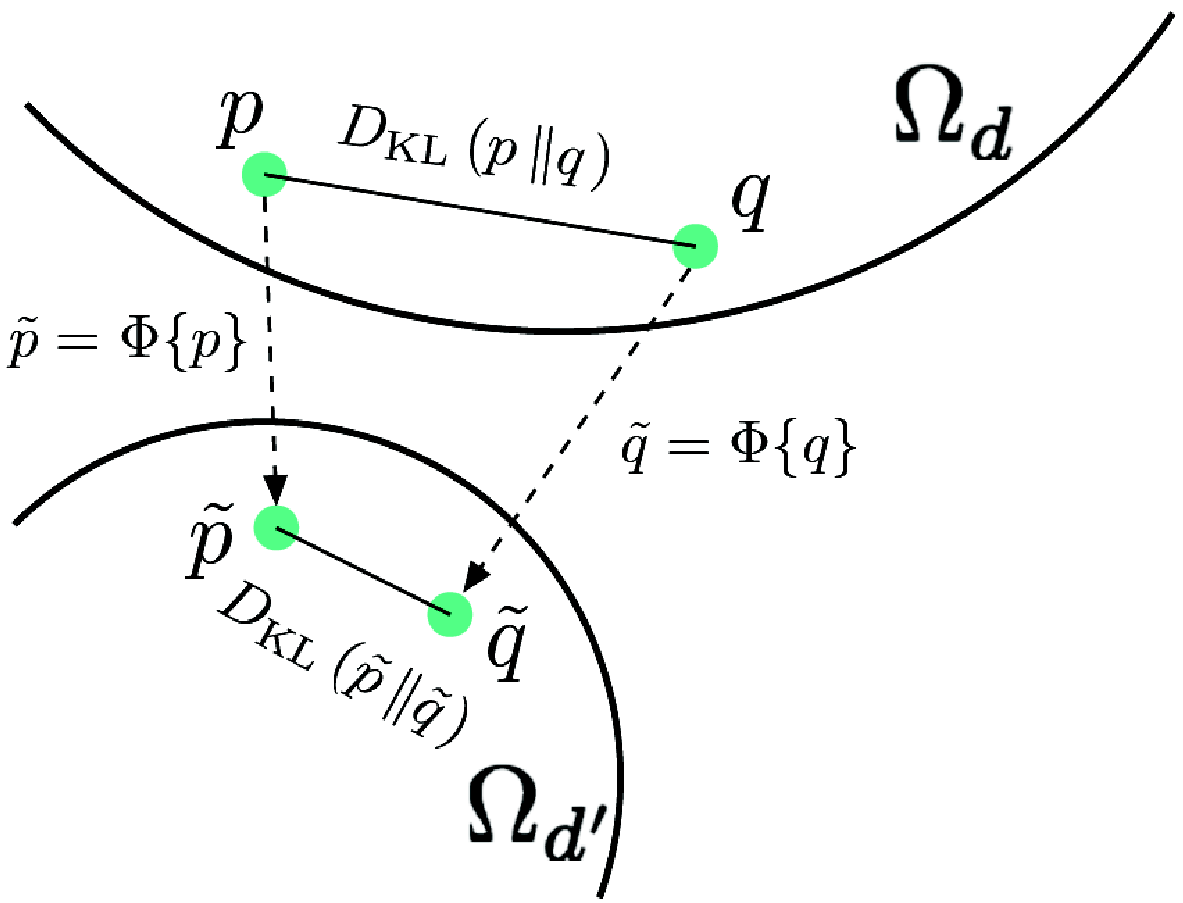
\includegraphics[width=.5\textwidth]{\fignet/Lyu11-Fig1} \text{\refer{Lyu11}}
  $$
  $\Phi: \Omega_d \mapsto \Omega_{d'}$ is KL-contactant iff, $\exists
  \beta \geq 1$, $\forall p, q \in \Omega_d$: 
  $$
  \emphase{KL[p ||q] - \beta \; KL[\Phi\{p\} ||\Phi\{q\}]} \geq 0.
  $$ 
}

%====================================================================
\frame{\frametitle{Examples of KL contraction} 

  
  \begin{itemize}
  \item \pause \emphase{Marginal distribution:} 
  $$
  {\Phi^m_a\{p\}(x) = \int p(x) \dd y_{\setminus a}.}
  $$\pause
  \item \emphase{Conditional distribution:} for a given distribution $t(y|x)$
  $$
  {\Phi^c_t\{p\}(y) = \int p(x) t(y|x) \dd x}.
  $$\pause
  \item \emphase{Marginal grafting:} replace $p_a(y^a)$ with $t_a(y^a)$
  $$
  \Phi^g_{t, a}\{p\}(x) = p(x)
  \frac{t_a(y^a)}{p_a(y^a)} = t_a(y^a) p_{\setminus a |a}(y^{\setminus a}| y^a).
  \pause
  $$
%   \item \emphase{Binary mixture:} $\displaystyle{\Phi^b_t\{p\}(x) =
%     \pi t(x) + (1 - \pi) p(x).}$ \\~ \pause
%   \item \emphase{Lumping} (= discretization): $\Scal = (S_1, \dots
%     S_m)$ a partition of $\mathbb{R}^d$,
%     $$
%     \Phi^\ell_\Scal\{p\}(i) = \int_{S_i} p(x) \dd x.
%     $$
  \item + binary mixture ($\approx$ shrinkage), lumping (= discretization), ...
  \end{itemize}

}

%====================================================================
\frame{\frametitle{Possible use for inference} 

  \begin{enumerate}[Type I:]
  \item Avoid to compute normalizing constants, which can vanish in
    the difference 
    \begin{equation} \label{Eq:DiffKL}
      KL[p ||q_\theta] - \beta \; KL[\Phi\{p\}||\Phi\{q_\theta\}]
    \end{equation} \\ \pause ~
  \item Define a easy-to-handle objective function based on a Taylor
    expansion of \eqref{Eq:DiffKL}. \\ \pause ~
  \item Use a set of contractions $(\Phi_1, \dots \Phi_A)$ to infer
    $\theta$ with
    $$
    \arg\min_\theta \sum_a w_a \left[KL[p||q_\theta] - \beta_a
      KL[\Phi_a\{p\}||\Phi_a\{q_\theta\}] \right].
    $$
  \end{enumerate}

  }

%====================================================================
\frame{\frametitle{Links with composite likelihoods} 

  \paragraph{Maximum likelihood:} Taking $p =$ empirical distribution and $q_\theta = $ parametric model,
  $$
  \widehat{\theta}_{ML} = \arg\min_\theta KL[p||q_\theta]
  $$

  \pause
  \paragraph{Type III with marginal contraction = Conditional composite 
    likelihood:}  
  For subsets $a_1, a_2, \dots$, using $\Phi_a^m$:
  $$
  \arg\max_\theta \sum_a w_a \log q_{\setminus a| a}(y^{\setminus a}|y^a; \theta) 
  $$
  \pause
  \paragraph{Type III with marginal grafting = Marginal composite likelihood:} using $\Phi_{p, a}^g$:
  $$
  \arg\max_\theta \sum_a w_a \log q_a(y^a; \theta)
  $$
  + Gaussian approximation using $\Phi^c_t$ where $t = \Ncal(x, \sigma^2)$.
  }

%====================================================================
\section{Conclusion?}
\frame{\frametitle{Outline} \tableofcontents[currentsection]}
%====================================================================
\frame{\frametitle{Conclusion: There is no conclusion} 

  \paragraph{Connexions do exist.} 
  \begin{itemize}
   \item Some variational approximations of the likelihood are actually
  composite likelihoods \refer{Lyu11,ZhS12}. 
  \item Many authors observe the connexion between composite likelihoods and (contrastive) divergence-based learning, but some end up using MCMC  \refer{LiJ08,ALI10,Fel14}...
  \end{itemize}
  
  \refer{Lyu11}: '{\em While many non-ML learning methods covered in this
  work have been shown to be consistent individually, the unification
  based on the minimum KL contraction may provide a general condition
  for such asymptotic properties.}' ...

  \pause
  \paragraph{But}
  \begin{itemize}
   \item No nice example to show
   \item Our favorite $KL[q_\theta || p]$ does not involve any contraction.
   \item No generic way to make the connexion.
  \end{itemize}

  }

%====================================================================
\frame{\frametitle{Variational/composite posterior as proposals}

  \paragraph{Approximate posterior.} Both variational Bayes and composite likelihood provide approximations of the posterior:
  $$
  p(\theta|y) \simeq q_{VB}(\theta),
  \qquad 
  p(\theta|y) \simeq q_{CL}(\theta) := p(\theta) e^{CL(y; \theta)}.
  $$

  \bigskip
  \paragraph{Importance sampling.} $q_{VB}$ and $q_{CL}$ can be used as proposal for importance sampling
  $$
  \widehat{\Esp}_p[f(\theta)|y] = \sum_b \frac{p(\theta^b, y)}{q(\theta^b)} f(\theta^b) \left/ \sum_b \frac{p(\theta^b, y)}{q(\theta^b)} \right.,
  \qquad \{\theta^b\} \text{ iid } \sim q
  $$
  but often lead too poor efficiency.
}  

%====================================================================
\frame{\frametitle{Calibrating variational/composite posteriors}

  Both variational Bayes and composite likelihood posterior need to be improved:
  $$
  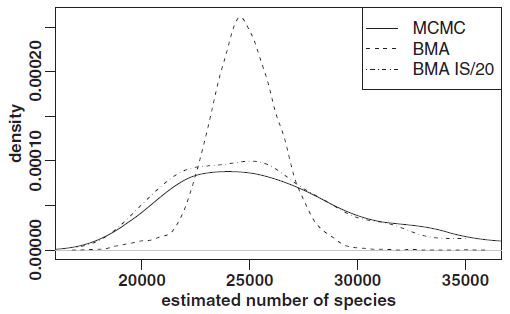
\includegraphics[width=.5\textwidth]{\figeco/LDR12-Fig6}
  $$
  
  Can we do that in a automated (sequential) way? Calibration: \refer{StF15}, Optimizing some efficiency criterion: \Refer{On-going work}.

}  

%====================================================================
%====================================================================
%\subsection*{References}
%====================================================================
{\tiny
  \bibliography{/home/robin/Biblio/ARC,/home/robin/Biblio/AST,/home/robin/Biblio/SSB}
%   \bibliographystyle{/home/robin/LATEX/Biblio/astats}
  \bibliographystyle{plain}
  }
  
%====================================================================
%====================================================================
\end{document}
%====================================================================
%====================================================================

